% Fonctionnement général de l'oscilloscope, prise en main, quelques manipulations pour observer le signal sur le microphone (en fonction du couplage, de l'amplitude, de l'échelle de temps...)

Assez d'explications théoriques, il est temps pour vous de passer à la pratique et d'essayer de mesurer les signaux produits par le microphone. Pour observer des signaux électriques, un instrument bien utile est l'oscilloscope. En connectant sa sonde (\textit{probe} en anglais) à un endroit du circuit, celui-ci affiche la tension en ce point au cours du temps. Il existe énormément de types d'oscilloscopes différents, des plus petits au plus complexes. Un oscilloscope est composé en général d'un écran sur lequel s'affiche le signal et de boutons de contrôle qui permettent de régler l'amplitude du signal affiché (en ordonnée sur le graphe) et l'échelle de temps (en abscisse). 

\begin{figure}[!ht]
	\centering
	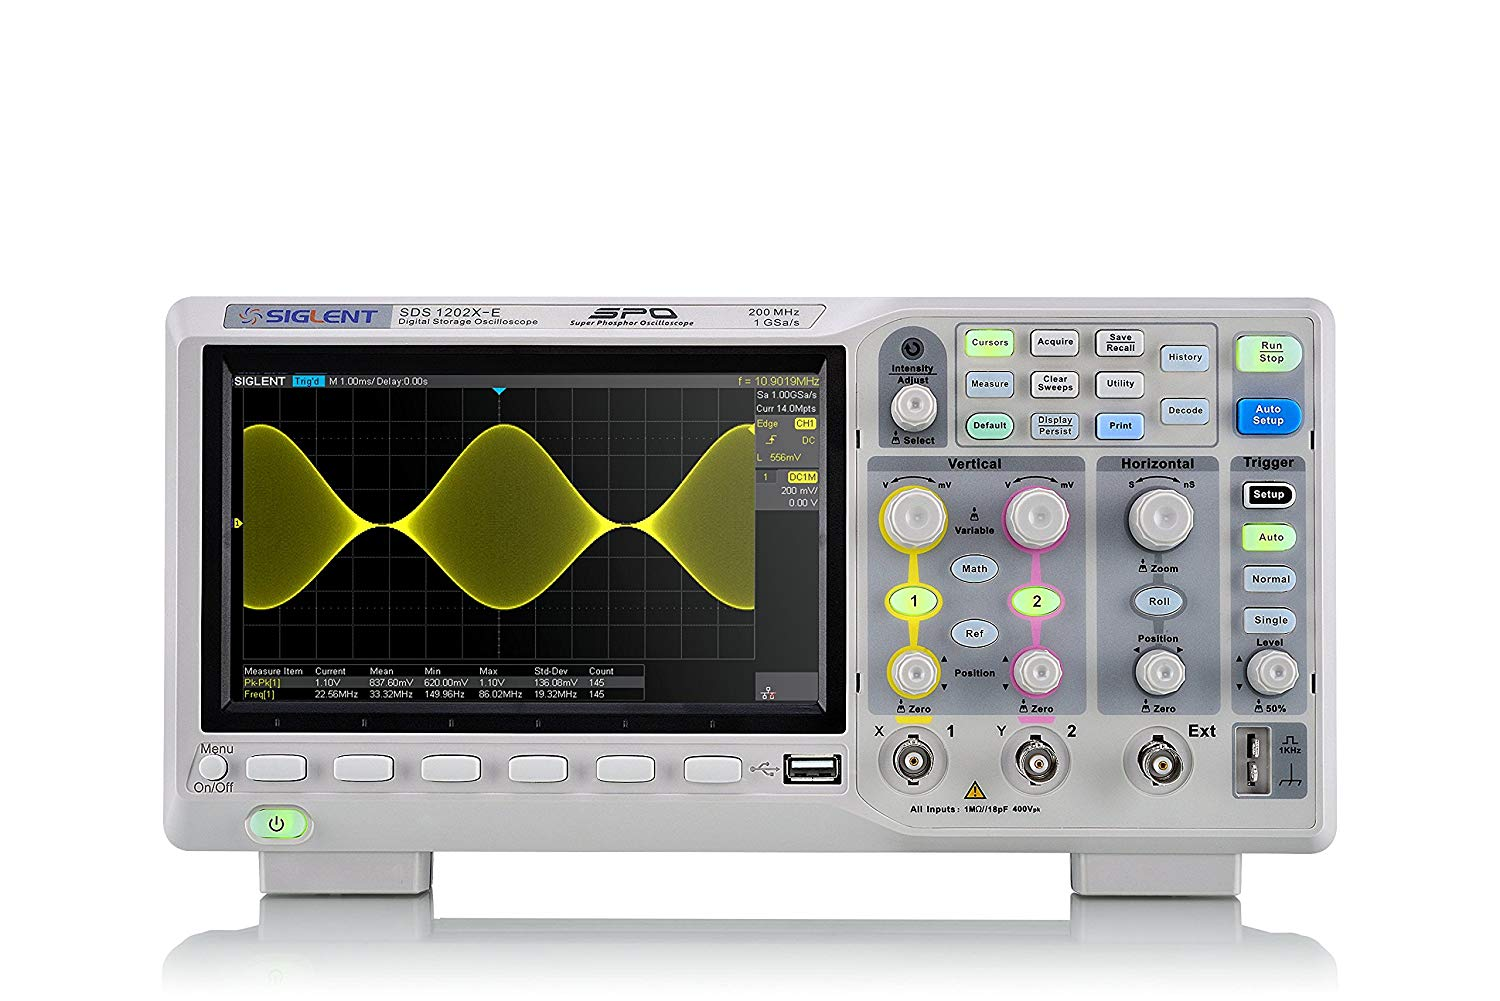
\includegraphics[width=.6\textwidth]{figures/oscillo.jpg}
	\caption{Oscilloscope}
	\label{fig:oscillo}
\end{figure}

L'affichage du signal fonctionne généralement en 2 modes différents: soit en mode continu où le signal défile sans arrêt sur l'écran, soit en mode déclenchable (\textit{trigger}) où le signal ne s'affiche que lorsqu'il dépasse un certain seuil. Ce deuxième mode est bien pratique pour observer des événements très brefs, tel que le signal sonore d'un claquement de doigts par exemple. \\

L'oscilloscope permet d'utiliser deux modes de couplage différents, appelés DC et AC (ça devrait te rappeler quelque chose...). Dans le mode DC, l'intégralité du signal est affiché à l'écran. \\

Les boutons correspondant à tous ces réglages sur chaque oscilloscopes sont différents d'une version à l'autre, appelle donc un membre du staff pour t'aider à t'y retrouver!\\

Pour chacun des signaux ci-dessous, réfléchis au réglage le plus approprié (amplitude, échelle de temps, mode continu ou déclenchable, découplage DC ou AC), et règle ensuite l'oscilloscope pour observer et mesurer le signal:
\begin{itemize}
\item La masse (référence de tension correspondant à 0V).
\item La tension d'alimentation à 5V.
\item La composante DC du signal de sortie du microphone.
\item La composante AC du signal de sortie du microphone.
\end{itemize}